% =============================================================================
% Supplemental Material — REVTeX 4.2 / PRL format (matches main.tex).
% Converted from the article-class version (preserved in
% supplementary_natcomp_backup.tex). Numeric APS citations (apsrev4-2);
% figures/equations/tables S-prefixed. BUILD ORDER: build both twice so the
% xr-hyper cross-refs between main.tex and supplementary.tex resolve.
% =============================================================================
\documentclass[
    aps,
    prl,
    reprint,
    superscriptaddress,
    amsmath,amssymb,
    nofootinbib,
    floatfix
]{revtex4-2}

\usepackage{graphicx}
\usepackage{bm}
\usepackage{xcolor}
\usepackage[colorlinks=true,allcolors=blue!50!black,citecolor=blue!50!black]{hyperref}
\usepackage{xr-hyper}                             % cross-refs to main-text labels
\externaldocument[M]{main}                            % reads main.aux
\usepackage{lineno}

\graphicspath{{./}{figures/}{SI_figures/}{img/}}

% Supplemental Material numbering (S-prefix)
\renewcommand{\thefigure}{S\arabic{figure}}
\renewcommand{\theequation}{S\arabic{equation}}
\renewcommand{\thetable}{S\arabic{table}}

\begin{document}

\title{End Matter (draft): A temporally-constrained latent space reveals the stochastic dynamics of convective organization}

\author{Sophie Abramian}
\affiliation{Department of Earth and Environmental Engineering, Columbia University, New York, NY, USA}

\author{Olivier Pauluis}
\affiliation{Courant Institute of Mathematical Sciences, New York University, New York, NY, USA}

\author{L. Ruby Leung}
\affiliation{Atmospheric Sciences and Global Change Division, Pacific Northwest National Laboratory, Richland, WA, USA}

\author{Pierre Gentine}
\affiliation{Department of Earth and Environmental Engineering, Columbia University, New York, NY, USA}

\date{\today}

\maketitle

\section{Per-state mass-flux profiles}

Let $M(h,z,t)$ denote the isentropic mass flux at time $t$, height $z$, and moist static energy $h$. For each cluster $c$, we define the cluster-mean vertically integrated positive and negative mass fluxes,
\begin{equation}
M^{\pm}_c(z)
=
\left\langle
\int_h M(h,z,t)\,\mathbf{1}\{\pm M>0\}
\right\rangle_{t\in c},
\end{equation}
and the anomalies relative to the simulation-wide mean profiles $\overline{M}^{\pm}(z)$,
\begin{equation}
\Delta^{\pm}_c(z)
=
M^{\pm}_c(z)-\overline{M}^{\pm}(z).
\end{equation}

\begin{figure*}[t]
    \centering
    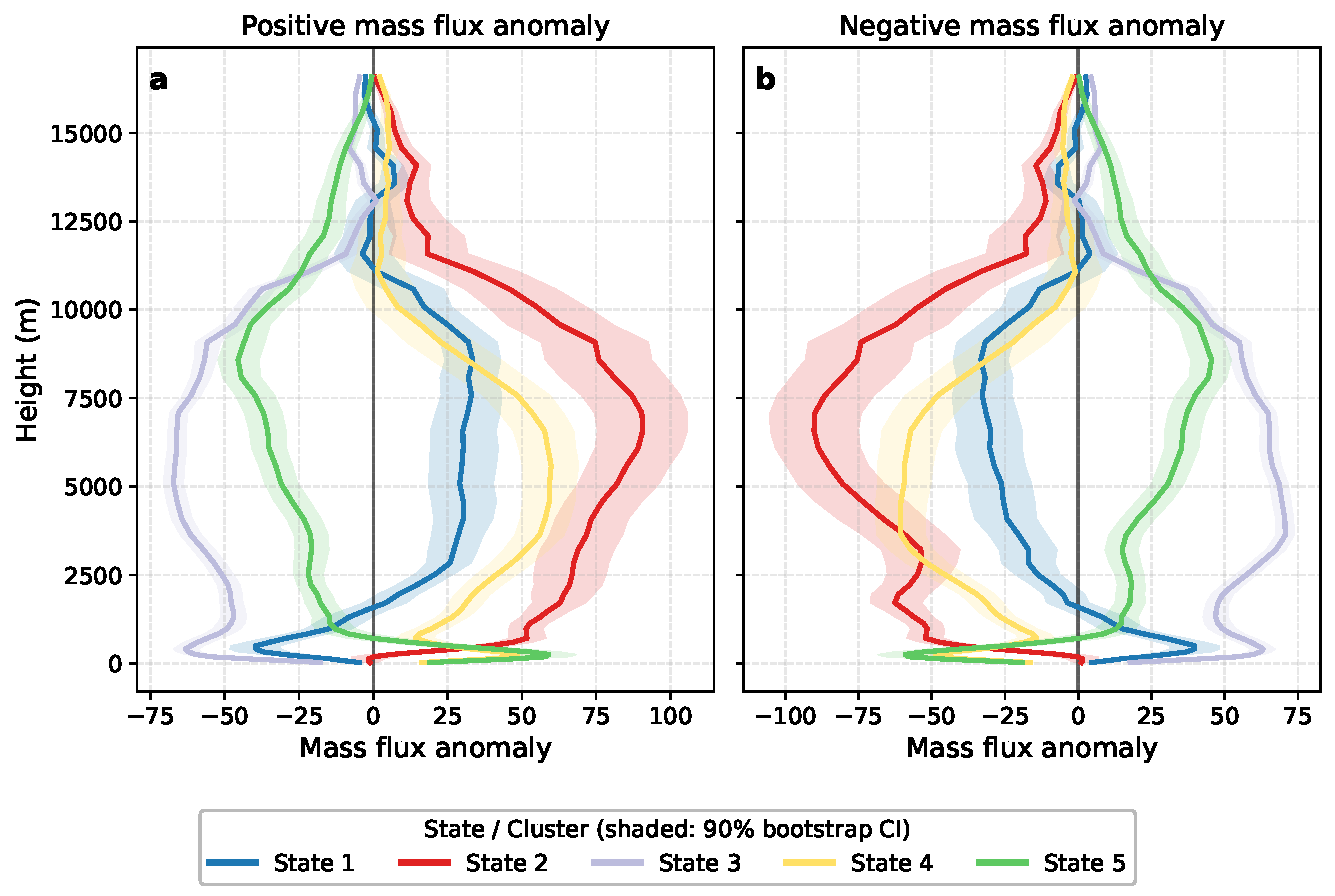
\includegraphics[width=0.36\textwidth]{fig5_vertical_profiles.pdf}\hfill
    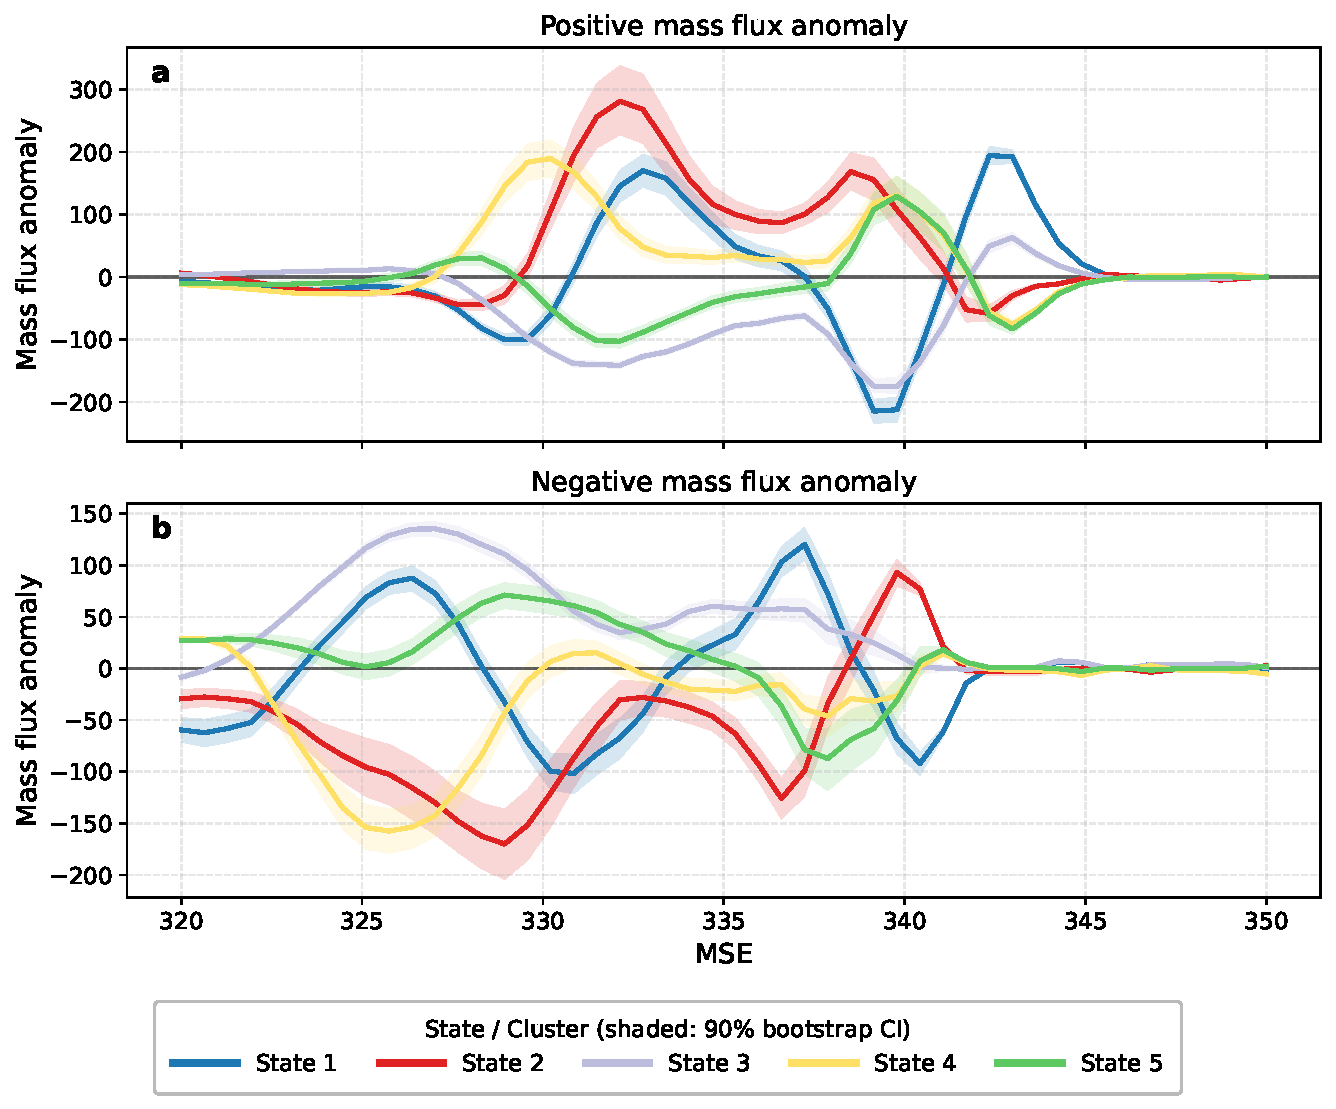
\includegraphics[width=0.36\textwidth]{fig6_mse_profiles.pdf}
    \caption{\textbf{State-averaged mass-flux anomalies.} \textbf{Left:} vertically resolved anomalies, \textbf{(a)}~positive (upward) and \textbf{(b)}~negative (downward). \textbf{Right:} the same anomalies resolved along moist static energy $\theta$. All are relative to the simulation-wide mean profile, computed from the samples closest to each state centroid in latent space; colours denote states (legend), solid lines the per-cluster mean, and shaded bands the 90\% bootstrap confidence interval.}
    \label{fig:profiles}
\end{figure*}

% --- Per-cluster vertical-profile description ---
The vertical profiles (Fig.~\ref{fig:profiles}, left) reveal sharp dynamical distinctions. State~1 has a deep upward anomaly with only a weak low-level downdraft, consistent with sustained deep ascent and suppressed detrainment; state~2 shows an even stronger upper-tropospheric ascent with the deepest mid-level downdraft, the signature of a mesoscale-stratiform system; state~4 peaks at lower altitude, characteristic of active but weakly organized convection; state~5 carries only shallow low-level ascent; and state~3 shows weak anomalies throughout.


% --- Per-cluster moist-static-energy description ---
Resolved along moist static energy (Fig.~\ref{fig:profiles}, right), the states separate thermodynamically. State~1 peaks at high $\theta\approx343$~K (warm, moist air lifted with reduced entrainment); state~2 spreads across $\theta\approx330$--$345$~K with its positive peak at intermediate $\theta$ (detrainment into a stratiform region); state~4 concentrates at lower $\theta\approx329$~K (less buoyant air, stronger entrainment); state~5 is confined to low--intermediate $\theta$; and state~3 lies below the mean throughout.



\section{Autocorrelation of state indicators in a Markov chain}

Let $\{X_t\}_{t\ge 0}$ be a stationary Markov chain on $\{1,\dots,K\}$ with transition matrix $\mathbf{T}$ and stationary distribution $\boldsymbol{\pi}$ ($\mathbf{T}\boldsymbol{\pi}=\boldsymbol{\pi}$, $\sum_i\pi_i=1$). For state $i$, the indicator $I_i(t)=\mathbb{1}[X_t=i]$ has mean $\mathbb{E}[I_i(t)]=\pi_i$, and we define the normalized autocorrelation
\begin{equation}
    C_i(\tau)
    =
    \frac{\mathbb{E}\!\left[(I_i(t)-\pi_i)(I_i(t+\tau)-\pi_i)\right]}
         {\mathbb{E}\!\left[(I_i(t)-\pi_i)^2\right]}.
    \label{eq:autocorr_def}
\end{equation}
Since $I_i$ is Bernoulli, the denominator is $\pi_i(1-\pi_i)$; by stationarity and the Markov property $\mathbb{E}[I_i(t)I_i(t+\tau)]=\pi_i(\mathbf{T}^\tau)_{ii}$. Hence
\begin{equation}
    C_i(\tau)=\frac{(\mathbf{T}^\tau)_{ii}-\pi_i}{1-\pi_i}.
\end{equation}
Writing the spectral decomposition $\mathbf{T}^\tau=\mathbf{1}\boldsymbol{\pi}^\top+\sum_{\alpha=2}^K\lambda_\alpha^\tau\,\mathbf{v}_\alpha\mathbf{w}_\alpha^\top$, with eigenvalues $1,\lambda_2,\dots,\lambda_K$ ($|\lambda_\alpha|<1$ for $\alpha\ge2$) and right/left eigenvectors $\mathbf{v}_\alpha,\mathbf{w}_\alpha$, the stationary term cancels and
\begin{equation}
    C_i(\tau)=\sum_{\alpha=2}^K A_\alpha^{(i)}\lambda_\alpha^\tau,
    \qquad
    A_\alpha^{(i)}=\frac{(\mathbf{v}_\alpha)_i(\mathbf{w}_\alpha)_i}{1-\pi_i}.
\end{equation}
At large lag the second eigenvalue dominates, $C_i(\tau)\sim\lambda_2^\tau=\exp(-\tau/\tau_{\mathrm{corr}})$ with $\tau_{\mathrm{corr}}=-1/\ln|\lambda_2|$: exponential decay of the state autocorrelations is a direct consequence of the Markov property.

\section{Cold-pool detection and activity index}

Cold pools, masses of cold, dense air that form below convective clouds through rain evaporation, are a key control on squall-line organization: they outlast the downdrafts that generate them and trigger or suppress new convection at their gust fronts \cite{rotunno1988theory, houze1977structure, tompkins2001coldpools, abramian2022shear, torri2015mechanisms}. In the main text they are identified as a candidate carrier of the memory that keeps the organized state~1 (and the active-unorganized state~4) alive beyond the Markov prediction. Testing this requires a time-resolved measure of cold-pool activity: we detect cold pools at each time step and summarize their total extent through a cold-pool index.

\subsection*{Cold-pool detection}

Cold pools are detected at each model time step from the two-dimensional surface temperature field $T_{abs}(x,y,t)$, smoothed with a Gaussian filter ($\sigma = 2$--$3$ grid points). Two thresholds define cold-pool envelopes ($T_{abs}<\phi_{\mathrm{env}}$) and their colder cores ($T_{abs}<\phi_{\mathrm{core}}<\phi_{\mathrm{env}}$). Envelope points are grouped into connected objects by single-linkage clustering with a periodic metric; core labels are propagated outward by nearest-neighbor classification, giving a labeled cold-pool mask at each step.


\subsection*{Cold-pool index}

A cold-pool index $\mathrm{CP}(t)$ is defined as the total area covered by cold pools at each time step,
\begin{equation}
\mathrm{CP}(t) = \sum_k A_k(t),
\end{equation}
where the sum runs over all cold pools present at time $t$. Normalized, anomalous, and standardized versions are also computed from its temporal mean and standard deviation.


\subsection*{Cold-pool conditioning of state-1 survival}

If cold pools carry the memory that keeps state~1 alive beyond the Markov prediction, then a state-1 configuration that \emph{already} carries a strong cold pool should behave \emph{more} Markovianly: much of the extra persistence is then explained by the cold pool that is present, so the state-1 autocorrelation should decay faster, back toward the Markov reference. We test this by conditioning on the cold-pool index at the starting time.

We first select the state-1 timesteps whose cold-pool index exceeds its 75th percentile $\mathrm{CP}_\star$,
\begin{equation}
J_1^\star(t)=\mathbf{1}\!\left[X_t=1\ \text{and}\ \mathrm{CP}(t)>\mathrm{CP}_\star\right],
\end{equation}
so that $J_1^\star(t)=1$ flags a ``strong--cold-pool'' start in state~1. For these starts we follow the \emph{survival} of state~1: the probability that the system is still in state~1 a lag $\tau$ later. The indicator $I_1(t+\tau)$ equals $1$ when $X_{t+\tau}=1$ and $0$ otherwise, so its conditional expectation given $J_1^\star(t)=1$---an average of $0$s and $1$s over the selected starts---is exactly the probability that the trajectory is back in (or still in) state~1 at lag $\tau$,
\begin{equation}
S^{(\mathrm{CP})}_1(\tau)=\mathbb{E}\!\left[\,I_1(t+\tau)\,\big|\,J_1^\star(t)=1\,\right].
\end{equation}
By construction $S^{(\mathrm{CP})}_1(0)=1$, since every selected trajectory starts in state~1; and at long lag the memory of the start is lost, so $S^{(\mathrm{CP})}_1(\tau)\to\pi_1$, the stationary occupancy of state~1. To place this survival on the same scale as the unconditional autocorrelation $C_1(\tau)$ of Eq.~\eqref{eq:autocorr_def}, which runs from $1$ at $\tau=0$ to $0$ at large lag, we subtract the baseline $\pi_1$ and divide by the available range $1-\pi_1$,
\begin{equation}
C^{(\mathrm{CP})}_1(\tau)=\frac{S^{(\mathrm{CP})}_1(\tau)-\pi_1}{1-\pi_1}.
\end{equation}
Subtracting $\pi_1$ sends the long-lag limit to $0$ and dividing by $1-\pi_1$ sends $\tau=0$ to $1$, mapping the survival from $[\pi_1,1]$ onto $[0,1]$ so it shares the axes of $C_1(\tau)$ and the Markov prediction (Fig.~\ref{Mfig:autocorrelation}b).

The condition is imposed \emph{only at the starting time} $t$; the trajectory then evolves freely---holding a cold pool in place throughout would force state~1 to persist and artificially truncate the survival, confounding the memory we seek to isolate.

\bibliographystyle{apsrev4-2}
\bibliography{biblio}

\end{document}